% !TeX spellcheck = en_US
\documentclass[aspectratio=1610]{beamer}
\usetheme{Madrid}
\setbeamercovered{transparent}
\setbeamertemplate{navigation symbols}{}
\setbeamertemplate{itemize items}[circle]
\setbeamertemplate{enumerate items}[default]

\makeatletter
\define@key{beamerframe}{wide}[10pt]{%
	\def\beamer@cramped{\itemsep #1\topsep0.5pt\relax}}
\makeatother
	

\usepackage[english]{babel}
\usepackage[utf8]{inputenc}
\usepackage[T1]{fontenc}
\usepackage{array}
\usepackage{xcolor}
\usepackage{colortbl}
\usepackage{booktabs}

\title[Winter - Lecture 6] % (optional, use only with long paper titles)
{Intermediate Macroeconomics: Lecture  W6 (Ch.13)}
\subtitle{ECON 311 -- Intermediate Macroeconomics}

\author{Muhebullah Karimzada}
\institute{School of Economics \\\ University of Northern British Columbia}
\date{Fall 2026}


% ---------- UNBC COLORS ----------
\usepackage{xcolor}
\definecolor{UNBCGreen}{RGB}{0,102,51}
\definecolor{UNBCDark}{RGB}{0,74,37}
\definecolor{UNBCGold}{RGB}{189,155,96}
\definecolor{SoftCream}{RGB}{249,247,242}
\definecolor{SoftGray}{RGB}{244,246,248}
\definecolor{AccentBlue}{RGB}{41,98,255}
\definecolor{AccentOrange}{RGB}{230,126,34}
\definecolor{AccentTeal}{RGB}{0,150,136}
\definecolor{AccentRed}{RGB}{192,57,43}
\setbeamercolor{normal text}{fg=black,bg=white}
\setbeamercolor{structure}{fg=UNBCDark}
\setbeamercolor{title}{fg=white,bg=UNBCDark}
\setbeamercolor{subtitle}{fg=UNBCGold}
\setbeamercolor{frametitle}{fg=white,bg=UNBCDark}
\setbeamercolor{block title}{fg=white,bg=UNBCDark}
\setbeamercolor{block body}{fg=black,bg=SoftGray}
\setbeamercolor{block title alerted}{fg=white,bg=AccentRed}
\setbeamercolor{block body alerted}{fg=black,bg=SoftGray}
\setbeamercolor{item}{fg=UNBCDark}
\setbeamercolor{section in toc}{fg=UNBCDark}
\setbeamercolor{alerted text}{fg=AccentRed}
\setbeamercolor{author in head/foot}{fg=white,bg=UNBCDark}
\setbeamercolor{date in head/foot}{fg=white,bg=UNBCDark}
% ---------- UNBC BRANDING ----------
\usepackage{graphicx}
\usepackage{lmodern}
\usepackage{tcolorbox}
\usepackage{tikz}
\usetikzlibrary{positioning,calc}
\setbeamertemplate{headline}{}
\setbeamertemplate{footline}{%
  \leavevmode%
  \hbox{%
  \begin{beamercolorbox}[wd=.78\paperwidth,ht=2.8ex,dp=1.2ex,leftskip=1em]{author in head/foot}%
  \color{white}\textbf{ECON 311} \hspace{0.5em} \textcolor{UNBCGold}{|} \hspace{0.5em} Intermediate Macroeconomics%
  \end{beamercolorbox}%
  \begin{beamercolorbox}[wd=.22\paperwidth,ht=2.8ex,dp=1.2ex,rightskip=1em plus1fil]{date in head/foot}%
  \color{white}\insertframenumber/\inserttotalframenumber%
  \end{beamercolorbox}}%
}

\newtcolorbox{mybox}[2][]{
  colback=#2!8,
  colframe=#2,
  boxrule=0.8pt,
  arc=2mm,
  left=2mm,right=2mm,top=1.5mm,bottom=1.5mm,
  #1
}

\newcommand{\topbanner}[1]{%
\begin{tikzpicture}[remember picture,overlay]
\fill[UNBCGold] ([yshift=-0.65cm]current page.north west) rectangle ([yshift=-0.48cm]current page.north east);
\node[anchor=north west,font=\small\bfseries,text=UNBCDark] at ([xshift=0.35cm,yshift=-0.78cm]current page.north west) {#1};
\end{tikzpicture}%
}
\begin{document}

\begin{frame}[plain]
  \titlepage
\end{frame}

\begin{frame}[wide]{What are You Going to Learn (Ch. 13)}
	\begin{itemize}
		\item The IS and MP curves combine to get the AD curve
		\vspace{2mm}
		\item The Phillips curve can be shown as the AS curve
		\vspace{2mm}
		\item Movements in the economy can be shown in the AS/AD model
		\vspace{2mm}
		\item Modern monetary policy theories
		\vspace{2mm}
		\item The appropriate policy response to shocks
	\end{itemize}
\end{frame}

\begin{frame}[wide]{Monetary Policy Rules and Aggregate Demand}
	Recall that:
	\begin{itemize}
		\vspace{2mm}
		\item IS Curve:
		\[\tilde{Y}_t = \bar{a} - \bar{b} \left(R_t -\bar{r}\right) \]
		\vspace{2mm}
		\item MP curve: Central bank pick $R_t$ exogenously - so far
		\vspace{2mm}
		\item Philips Curve: 
		\[\Delta \pi_t = \bar{\nu} \tilde{Y}_t +\bar{o}\]
		\vspace{2mm}
		\item This model implies high short-run output ($\tilde{Y}_t$) increases inflation ($\Delta \pi_t>0$)
		\vspace{2mm}
		\item The central bank faces this trade-off and chooses the interest rate
	\end{itemize}
\end{frame}

\begin{frame}[wide]{Simple Monetary Policy Rule}
	\begin{itemize}
		\item A monetary policy rule is a guideline for central bankers under certain economic circumstances, when output or inflation changes
		\vspace{2mm}
		\item The following simple rule have the real interest rate a function of the inflation rate:
		\vspace{2mm}
		\begin{itemize}
			\item If inflation is high (low), the interest rate should increase (decrease)
		\end{itemize}
		\vspace{2mm}
		\[R_t - \bar{r} = \bar{m} \left(\pi_t - \bar{\pi}\right)\]
		\item The new component is 
		\vspace{2mm}
		\begin{itemize}
			\item $\bar{\pi}$: Inflation target
			\vspace{2mm}
			\begin{itemize}
				\item As of now, Canada, the United States, United Kingdom, euro area, and Japan all have an explicit target of 2 percent
				\item Treat it as the steady-state rate of inflation 
			\end{itemize}
			\vspace{2mm}
			\item $\bar{m}$: dictates how aggressively monetary policy responds to inflation
		\end{itemize}
	\end{itemize}
\end{frame}

\begin{frame}[wide]{The AD Curve}
	\begin{itemize}
		\item Put together the IS curve and the policy rule (sub in $R_t - \bar{r}$)
		\[\tilde{Y} = \bar{a} - \bar{b} \bar{m} \left(\pi_t - \bar{\pi}\right)\]
		\vspace{2mm}
		\item Short-run output is a function of the inflation rate
		\vspace{2mm}
		\item Invert the equation:
		\[\tilde{Y} - \bar{a} = -\bar{b}\bar{m} \left(\pi_t - \bar{\pi}\right)\]
		\[\frac{\tilde{Y} - \bar{a}}{-\bar{b}\bar{m}} =  \left(\pi_t - \bar{\pi}\right)\]
		\[\pi_t  = \frac{\tilde{Y} - \bar{a}}{-\bar{b}\bar{m}} + \bar{\pi} = \frac{ \bar{a}}{\bar{b}\bar{m}}+ \bar{\pi} - \frac{1}{\bar{b}\bar{m}} \tilde{Y}\]
	\end{itemize}
\end{frame}

\begin{frame}[wide]{The AD Curve}
	\begin{itemize}
		\item If inflation is above (below) its target, the Central Bank raises (falls) rates and	output falls (rises) below potential
	\end{itemize}
	\begin{figure}
		\centering
		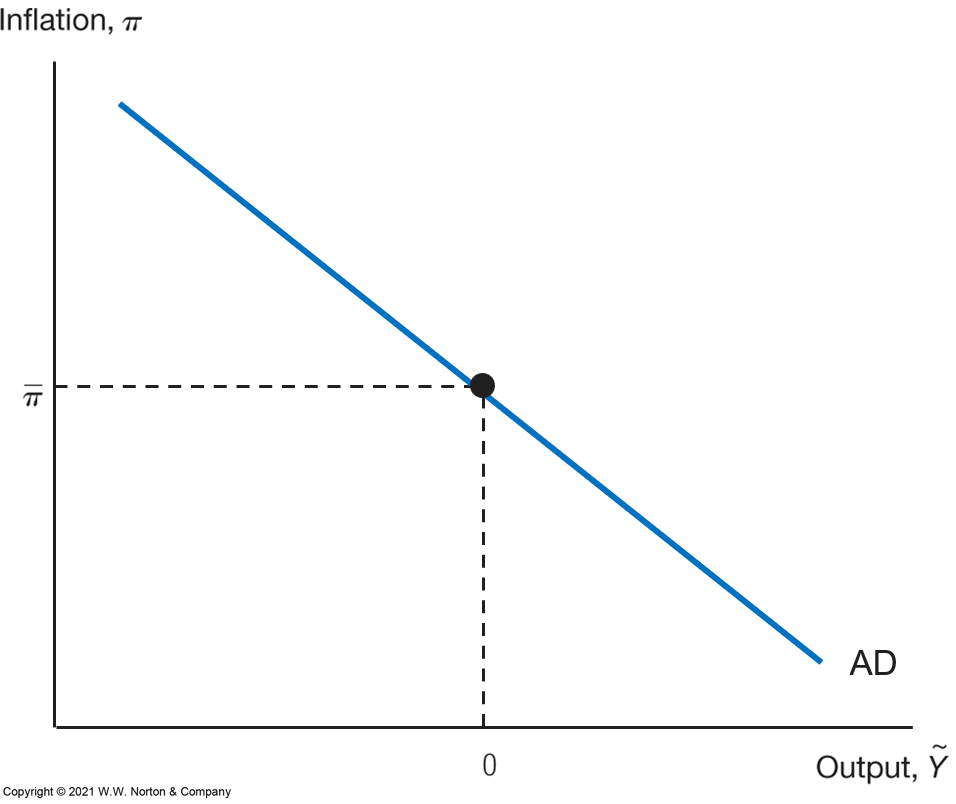
\includegraphics[width=0.55\linewidth]{Figures/fig_13_01}
	\end{figure}
\end{frame}

\begin{frame}[wide]{The AD Curve}
	\begin{itemize}
		\item The AD curve combine the central bank's choice of the interest rate, and, consequently, short-run output, based on the current inflation rate 
		\vspace{4mm}
		\begin{itemize}
			\item Change in inflation: a movement along the AD curve
			\vspace{5mm}
			\item Change in $\bar{m}$: change the slope of the AD curve
			\vspace{5mm}
			\item Changes in the parameter $\bar{a}$ or $\bar{\pi }$: 			AD curve shifts
		\end{itemize}
	\end{itemize}
\end{frame}

\begin{frame}[wide]{The AD Curve after an Inflation Shock}
	\begin{itemize}
		\item Seeing an increase in inflation, the monetary policy rule dictates that the central bank increase the interest rate, thereby reducing short-run output
	\end{itemize}
	\begin{figure}
		\centering
		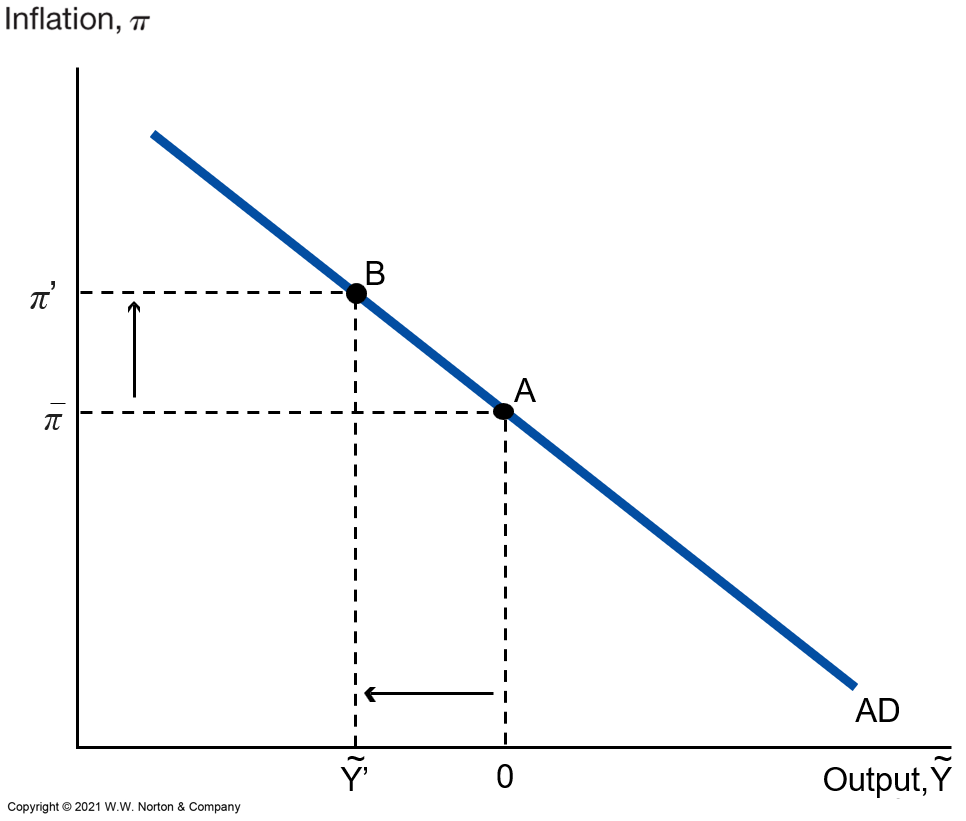
\includegraphics[width=0.5\linewidth]{Figures/fig_13_02}
	\end{figure}
	
\end{frame}

\begin{frame}[wide]{An Aggressive Monetary Policy Rule}
	\begin{itemize}
		\item A high value of $\bar{m}$ means the monetary policy rule produces a large recession in order to fight a given increase in the inflation rate
		\item A one-percentage-point increase in the inflation rate dictates a large decline in short-run output
	\end{itemize}
	\begin{figure}
		\centering
		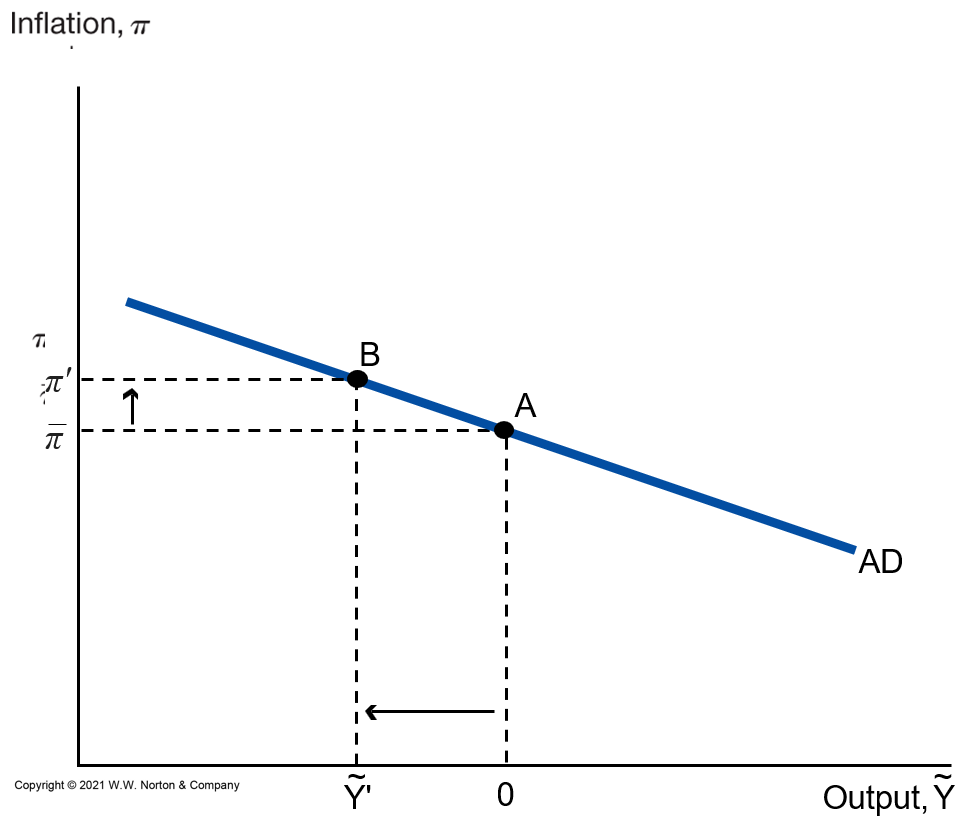
\includegraphics[width=0.45\linewidth]{Figures/fig_13_03}
	\end{figure}
\end{frame}

\begin{frame}[wide]{The Aggregate Supply Curve}
	\begin{itemize}
		\item The Phillips curve  relates the current rate of inflation to short-run output
		\vspace{4mm}
		\begin{itemize}
			\item It describe the price-setting equation used by firms in the economy
			\item Also, firms supply good and services
		\end{itemize}
		\vspace{2mm}
		\[\pi_t = \pi_{t-1} +\bar{\nu} \tilde{Y}_t + \bar{o}\]
		\vspace{2mm}
	
	\end{itemize}
\end{frame}

\begin{frame}[wide]{The Aggregate Supply Curve}
	\begin{itemize}
		\item When there are no inflation shocks ($\bar{o} = 0$) and when output is at potential ($\tilde{Y}=0$), firms simply expect the current rate of inflation to prevail (i.e., $\pi_t = \pi_{t-1}$)
		\vspace{6mm}
		\item The AS curve will shift due to
		\vspace{4mm}
		\begin{itemize}
			\item change in $\tilde{Y}$
			\begin{itemize}
				\item Higher output today leads firms to raise their prices by more, which increases inflation today and tomorrow
			\end{itemize}
			\vspace{2mm}
			\item change in the inflation shock parameter
		\end{itemize}
		\vspace{4mm}
		\item These shock would carry over to future period until another shock cancel out the effect
	\end{itemize}
\end{frame}

\begin{frame}[wide]{The Aggregate Supply Curve}
	
	\begin{figure}
		\centering
		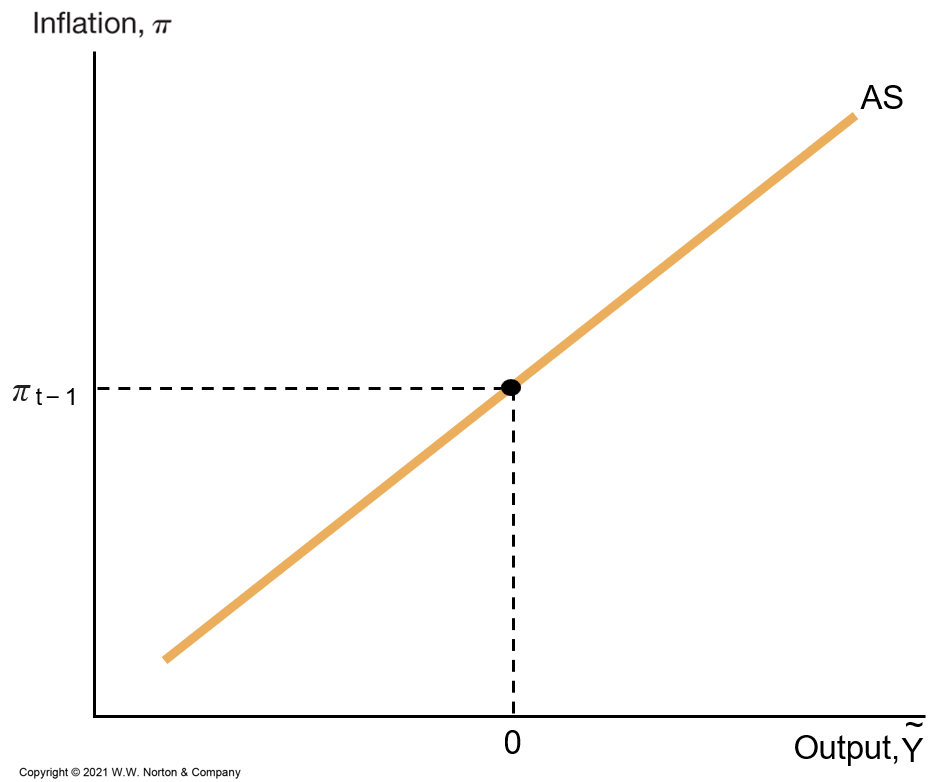
\includegraphics[width=0.5\linewidth]{Figures/fig_13_04}
	\end{figure}
\end{frame}

\begin{frame}[wide]{The AS/AD Framework}
	\begin{itemize}
		\item Combining the AS and AD curve
		\vspace{4mm}
		\item Two equation: AS and AD
		\vspace{4mm}
		\item Two unknowns: inflation rate and short-run output
		\vspace{2mm}
		\[\tilde{Y} = \bar{a} - \bar{b} \bar{m} \left(\pi_t - \bar{\pi}\right)\]
		\[\pi_t = \pi_{t-1} + \bar{\nu} \tilde{Y}_t + \bar{o}\]
	\end{itemize}
\end{frame}


\begin{frame}[wide]{The Steady State}
	\begin{itemize}
		\item We will first start with steady state, then study the dynamic of the model
		\vspace{3mm}
		\item In the steady state
		\vspace{2mm}
		\begin{itemize}
			\item The endogenous variables are constant over time (i.e., $\pi_t =\pi_{t-1} = \pi^*, \tilde{Y} = 0$)
			\item No shocks to the economy (i.e., $\bar{o} = 0, \bar{a} = 0$)
		\end{itemize}
		\vspace{3mm}
		\item Starting with the AS curve (let $\pi_t=\pi_{t-1} = \pi^*$):
		\vspace{2mm}
		\[\bar{\pi} = \bar{\pi} + \bar{\nu} \tilde{Y}_t  \implies 0 = \bar{\nu} \tilde{Y} \]
		\[ \tilde{Y} = 0\]
		\vspace{1mm}
		\item The AS curve is consistent with the steady state
	\end{itemize}
\end{frame}

\begin{frame}[wide]{The Steady State}
	\begin{itemize}
		\item From the AD curve ($\tilde{Y}= 0 $ and $\bar{a} = 0 $)
		\vspace{2mm}
		\[\tilde{Y}_t = \bar{a} - \bar{b}\bar{m} \left(\pi_t - \bar{\pi}\right)\]
		\[0 = 0 - \bar{b}\bar{m} \left(\pi_t - \bar{\pi}\right)\]
		\vspace{2mm}
		\item This implies 
		\vspace{2mm}
		\[\pi_t=\pi_{t-1}=\bar{\pi}\]
		\vspace{2mm}
		\item AD curve is also consistent with the steady state
	\end{itemize}
\end{frame}

\begin{frame}[wide]{The AS/AD Framework}
	\begin{figure}
		\centering
		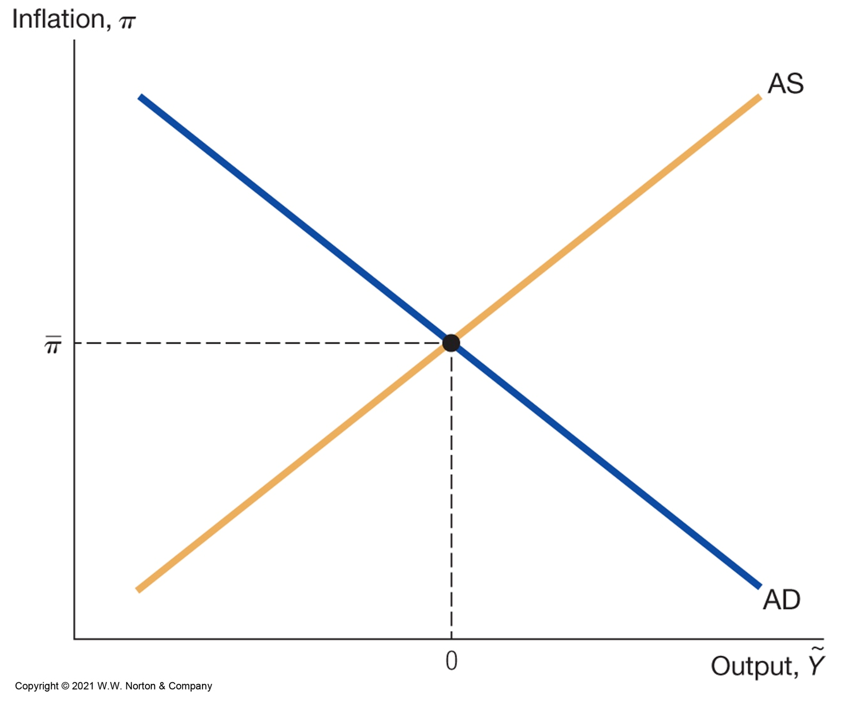
\includegraphics[width=0.5\linewidth]{Figures/fig_13_05}
	\end{figure}
\end{frame}

\begin{frame}[wide]{Macroeconomic Events: Event 1—An Inflation Shock}
	\begin{itemize}
		\item Unless specific otherwise, the economy begins in steady state
		\vspace{5mm}
		\item Suppose there is a increase oil price for one period
		\vspace{2mm}
		\begin{itemize}
			\item The parameter $\bar{o}$ is positive for one period
			\item The inflation rises
			\item The AS curve will shift up as a result
		\end{itemize}
		\vspace{5mm}
		\item The monetary policy rule states that the increase in inflation be fought by an increase in the real interest rate, reducing short-run output
		
		
	\end{itemize}
\end{frame}

\begin{frame}[wide]{The Initial Response to an Inflation Shock}
	
	\begin{figure}
		\centering
		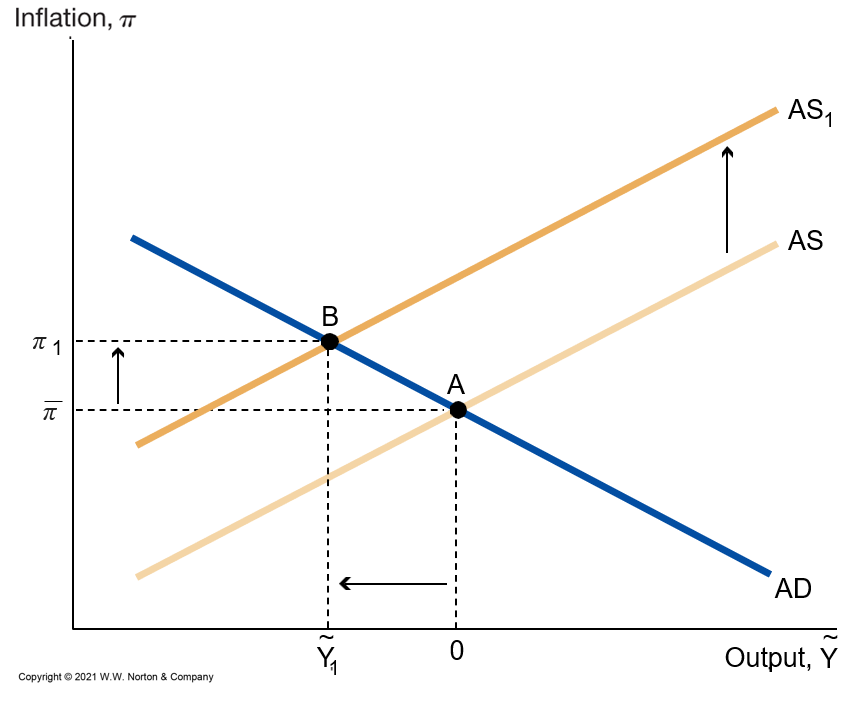
\includegraphics[width=0.5\linewidth]{Figures/fig_13_06}
	\end{figure}
	\begin{itemize}
		\item Stagflation:	Combination of a recession and inflation
		\item But, that is just the initial impact 
	\end{itemize}
\end{frame}

\begin{frame}[wide]{Event 1: An Inflation Shock}
	\begin{itemize}
		\item In period 1, the inflation would be 
		\[\pi_1 = \bar{\pi} + \bar{\nu} \tilde{Y}_1 + \bar{o}\]
		\item In period 2, $\bar{o}$ return to zero, the AS curve is now: 
		\[\pi_2 = \pi_1 + \bar{\nu}\tilde{Y}_2 = \bar{\pi} + \bar{\nu} \tilde{Y}_1 + \bar{o} + \bar{\nu}\tilde{Y}_2\]
		\item Since $\pi_1 > \bar{\pi}$, the AS curve is not back to steady state
		\begin{itemize}
			\item Note the term $\tilde{Y}_1 $ and $\tilde{Y}_2$ are negative
			\item This implies the inflation would get lower and lower over time!!
		\end{itemize}
	\end{itemize}
\end{frame}

\begin{frame}[wide]{Event 1: An Inflation Shock}
	\begin{itemize}
		\item In word,
		\vspace{4mm}
		\begin{itemize}
			\item High inflation from the oil shock
			\item It rises the expected inflation
			\item AS curve does not adjust back to steady state right away
			\item As seen next, inflation slowly falls and model return to its steady state
		\end{itemize}
	\end{itemize}
\end{frame}

\begin{frame}[wide]{Two Periods after an Inflation Shock}
	\begin{itemize}
		\item Because of sticky prices, high inflation expectations adjust only slowly
		\item At $\tilde{Y} = 0$, the AS curve would shift down a bit from $AS_1$
	\end{itemize}
	\vspace{5mm}
	\begin{figure}
		\centering
		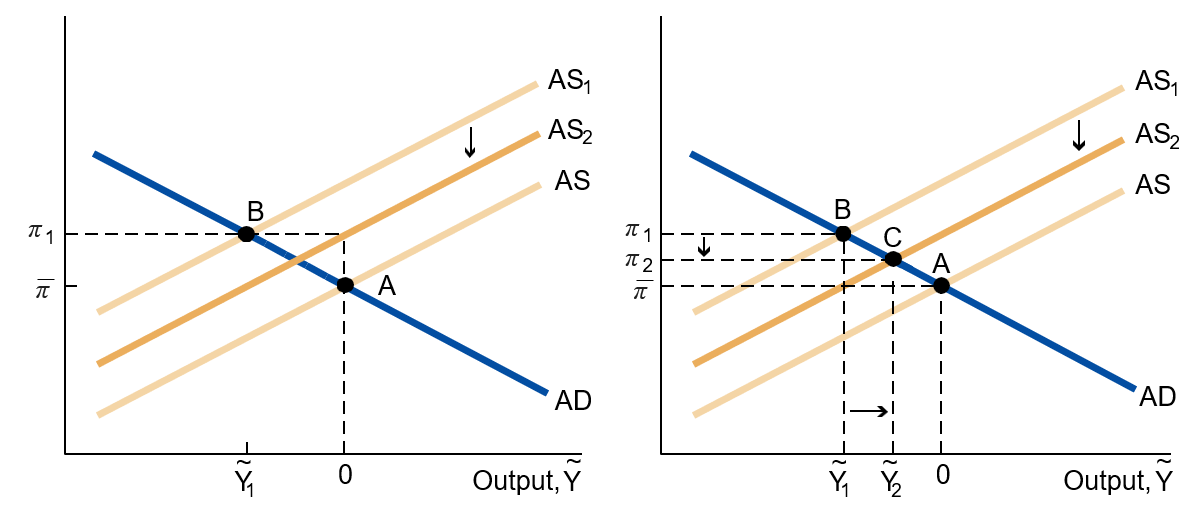
\includegraphics[width=0.8\linewidth]{Figures/fig_13_07}
	\end{figure}
\end{frame}

\begin{frame}[wide]{Three Periods after an Inflation Shock}
	\begin{itemize}
		\item In period three, expected inflation falls further, shifting the AS curve closer to its original position
		\item Eventually, the AS curve would move back to the steady state position
	\end{itemize}
	\begin{figure}
		\centering
		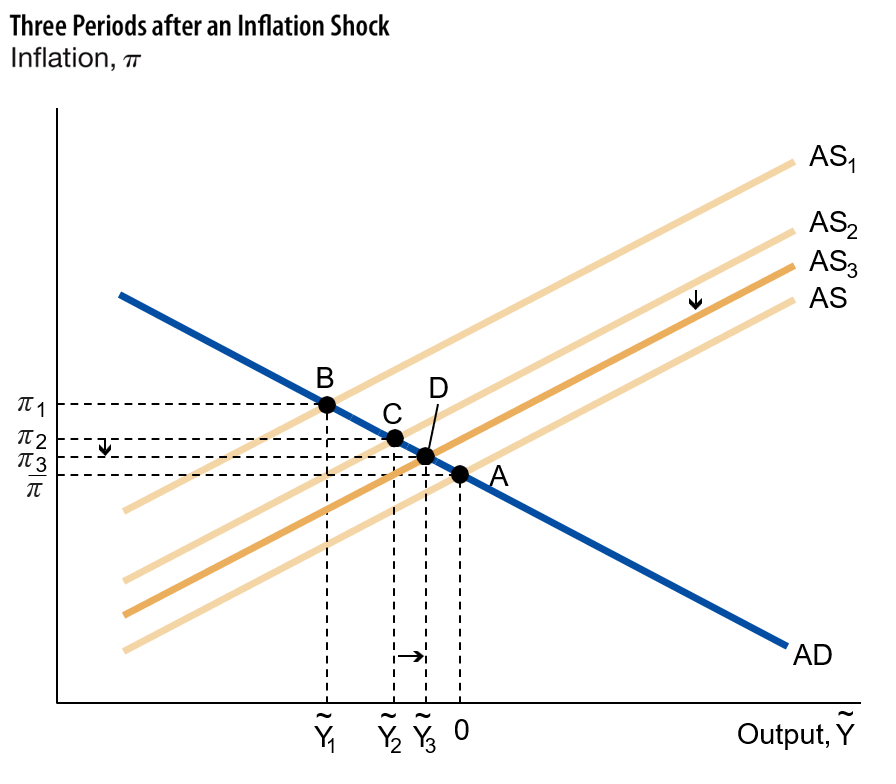
\includegraphics[width=0.5\linewidth]{Figures/fig_13_08}
	\end{figure}
\end{frame}

\begin{frame}[wide]{Event 1: An Inflation Shock}
	\begin{itemize}
		\item What we have just saw is similar to the principle of transition dynamics, which we encountered in the long-run model
		\vspace{4mm}
		\item Another note is that the movement back to the steady state is fastest when the economy is furthest from its steady state
		\vspace{4mm}
		\item In summary, a price shock
		\vspace{2mm}
		\begin{itemize}
			\item raises inflation directly
			\item the central bank induces a recession to fight inflation
			\item keeps inflation higher for a longer period of time due to sticky inflation
			\item results in a prolonged slump
			\item causes the economy to suffer from stagflation
		\end{itemize}
	\end{itemize}
\end{frame}

\begin{frame}[wide]{The Effects of an Inflation Shock}
	\begin{itemize}
		\item As expected inflation declines gradually, causing the AS curve to shift back toward its original position
		\item Sticky inflation assumption is at the heart of this gradual adjustment
	\end{itemize}
	\begin{figure}
		\centering
		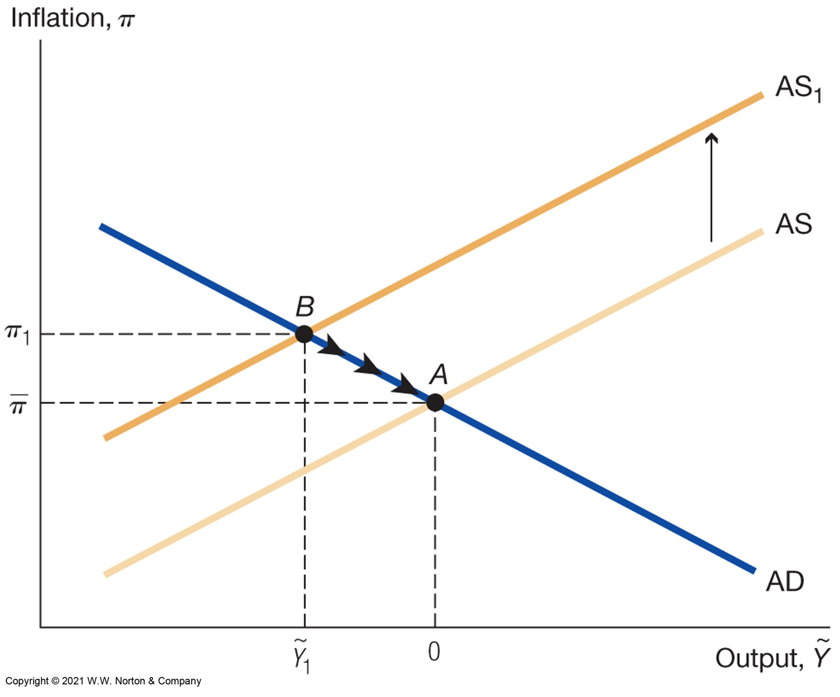
\includegraphics[width=0.5\linewidth]{Figures/fig_13_09}
	\end{figure}
	
\end{frame}

\begin{frame}[wide]{Event 2: Disinflation}
	\begin{itemize}
		\item Suppose policymakers decide to lower the inflation target.
		\vspace{4mm}
		\begin{itemize}
			\item The AD curve shifts down, as $\bar{\pi}$ falls
			\[\tilde{Y}_t = \bar{a} -\bar{b} \bar{m} \left(\pi_t - \textcolor{red}{\bar{\pi}}\right)\]
			\item The new rule calls for an increase in interest rates
			\[R_t - \bar{r} = \bar{m} \left(\pi_t - \textcolor{red}{\bar{\pi}}\right)\]
		\end{itemize}
	\end{itemize}
\end{frame}

\begin{frame}[wide]{The Initial Response to Disinflation}
	\begin{itemize}
		\item The reduction in the inflation target shifts the AD curve down
	\end{itemize}
	\begin{center}
		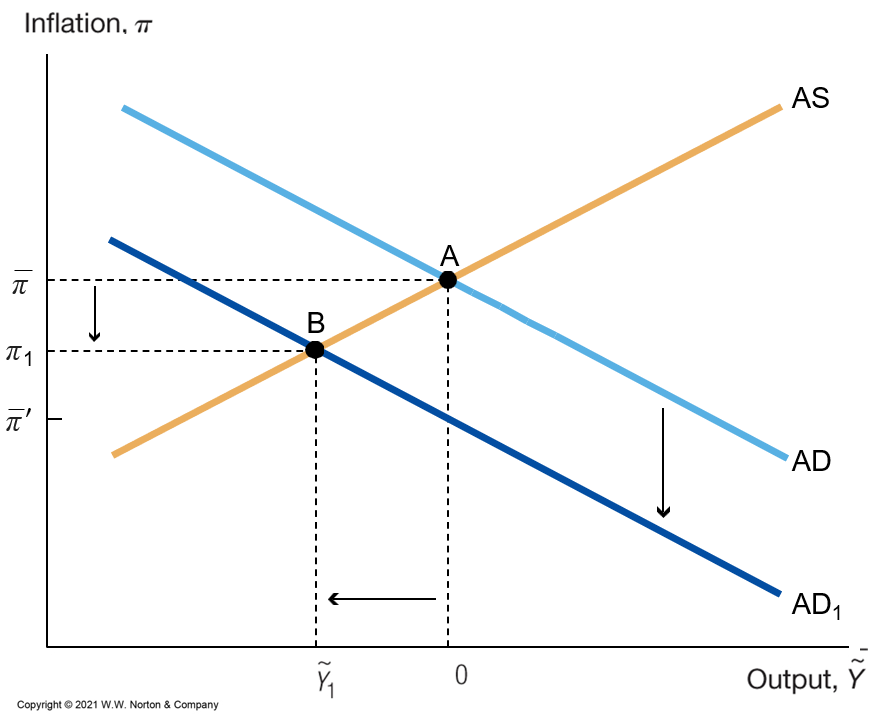
\includegraphics[width=0.5\linewidth]{Figures/fig_13_10}
	\end{center}
\end{frame}

\begin{frame}[wide]{The Dynamics of Disinflation}
	\begin{itemize}
		\item We can apply the principle of transition dynamics
		\item Here, the change in the monetary policy rule means that the steady-state rate of inflation has now changed
	\end{itemize}
	\begin{center}
		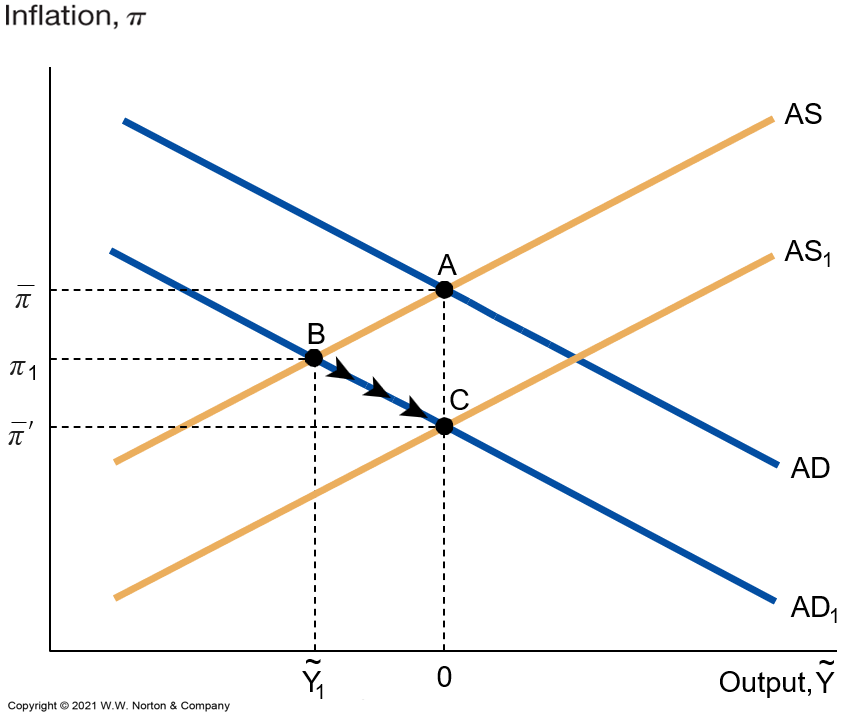
\includegraphics[width=0.5\linewidth]{Figures/fig_13_11}
	\end{center}
\end{frame}

\begin{frame}[wide]{Event 2: Disinflation }
	\begin{itemize}
		\item If the classical dichotomy holds in the short run, the AD and AS curves would reach the new steady state immediately
		\vspace{6mm}
		\item But there is a sticky inflation. A recession is needed to adjust expectations down
		\vspace{6mm}
		\item In the process of changing a monetary policy rule, the credibility of policymakers and the way price setters form their expectations play critical roles
		\vspace{3mm}
		\begin{itemize}
			\item Michelle Alexopoulos (at U of T) and her co-authors analyze effect U.S. Federal Reserve Chairs's word, voice and facial expression when deliver congressional testimonies  on financial markets (JME 2024)
		\end{itemize}
	\end{itemize}
\end{frame}

\begin{frame}[wide]{Event 2: Disinflation }
	\begin{itemize}
		\item Summary:
		\vspace{2mm}
		\begin{itemize}
			\item The policy change lead to a downward shift of the AD curve
			\vspace{2mm}
			\item The change in the rate of inflation causes the AS curve to shift in the following period
			\vspace{2mm}
			\begin{itemize}
				\item Firms adjust their expectation for inflation to account for the new lower inflation rate
			\end{itemize}
			\vspace{2mm}
			\item The inflation rate is still above the target, the central bank keeps actual output below potential
			\vspace{2mm}
			\item Eventually, as inflation rate falls further, the economy will rest in its new steady state
		\end{itemize}
	\end{itemize}
\end{frame}

\begin{frame}[wide]{Event 3: A Positive AD Shock}
	\begin{itemize}
		\item Suppose there is a temporary increase in the aggregate demand parameter, $\bar{a}$
		\item The AD curve will shift out
		\begin{itemize}
			\item Increased demand lead to an increase in prices
		\end{itemize}
		\begin{center}
			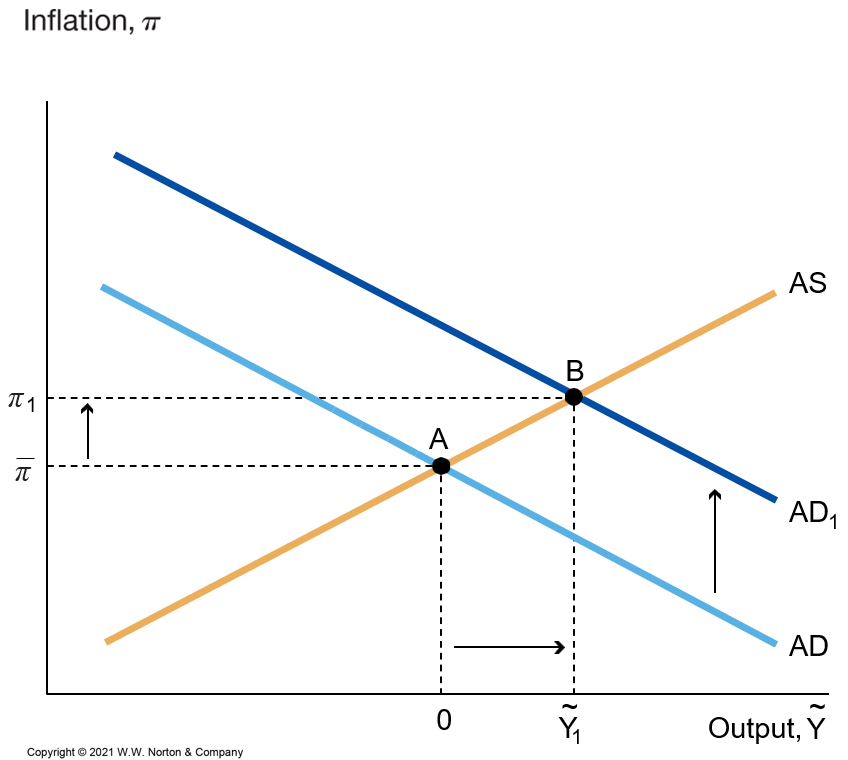
\includegraphics[width=0.5\linewidth]{Figures/fig_13_12}
		\end{center}
		
	\end{itemize}
\end{frame}

\begin{frame}[wide]{Event 3: A Positive AD Shock}
	\begin{itemize}
		\item Following the increase in demand (i.e., $\bar{a}$ increases), firms raise prices.
		\begin{itemize}
			\item Inflation increases
		\end{itemize}
		\item As the inflation rise, AS curve shift up 
		\item Short-run output  return to zero gradually
		\begin{center}
			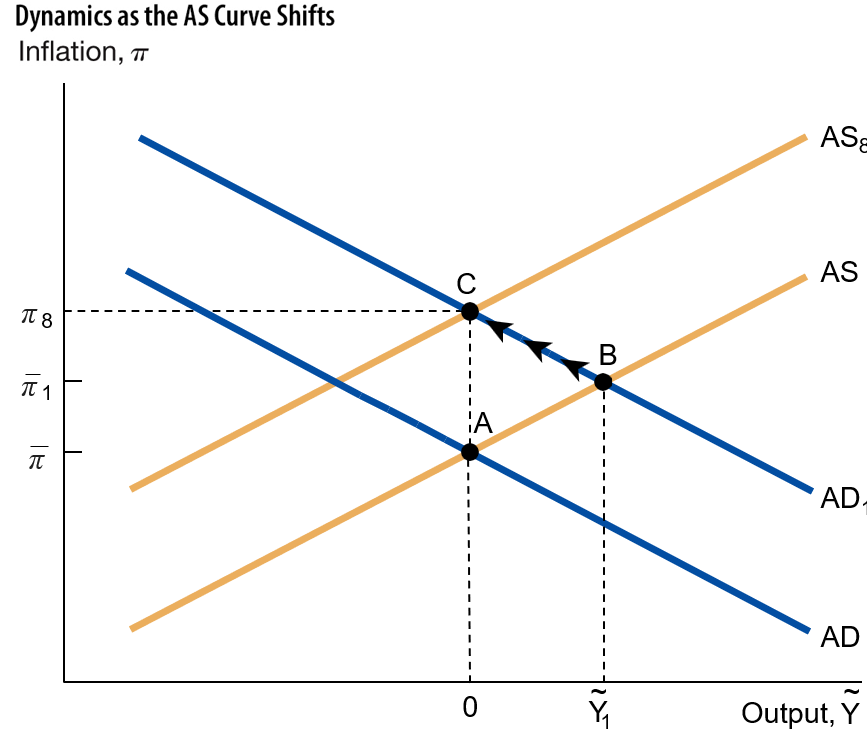
\includegraphics[width=0.45\linewidth]{Figures/fig_13_13}
		\end{center}
		
	\end{itemize}
\end{frame}

\begin{frame}[wide]{The Unraveling after the AD Shock Ends}
	\begin{itemize}
		\item Recall, aggregate demand shocks are temporary. In the long run, $\bar{a} = 0$ 
		\vspace{5mm}
		\item When the shock ends, the AD curve shifts back to its original position
		\vspace{2mm}
		\begin{itemize}
			\item  This is much like a negative shock because short-run output was already at 0
		\end{itemize}
		\vspace{5mm}
		\item The shift back to its original position puts downward pressure on inflation:
		\vspace{2mm}
		\begin{itemize}
			\item Transition dynamics returns the economy to steady state as the AS curve shifts
		\end{itemize}
	\end{itemize}
\end{frame}

\begin{frame}[wide]{The Unraveling after the AD Shock Ends}
	\begin{center}
		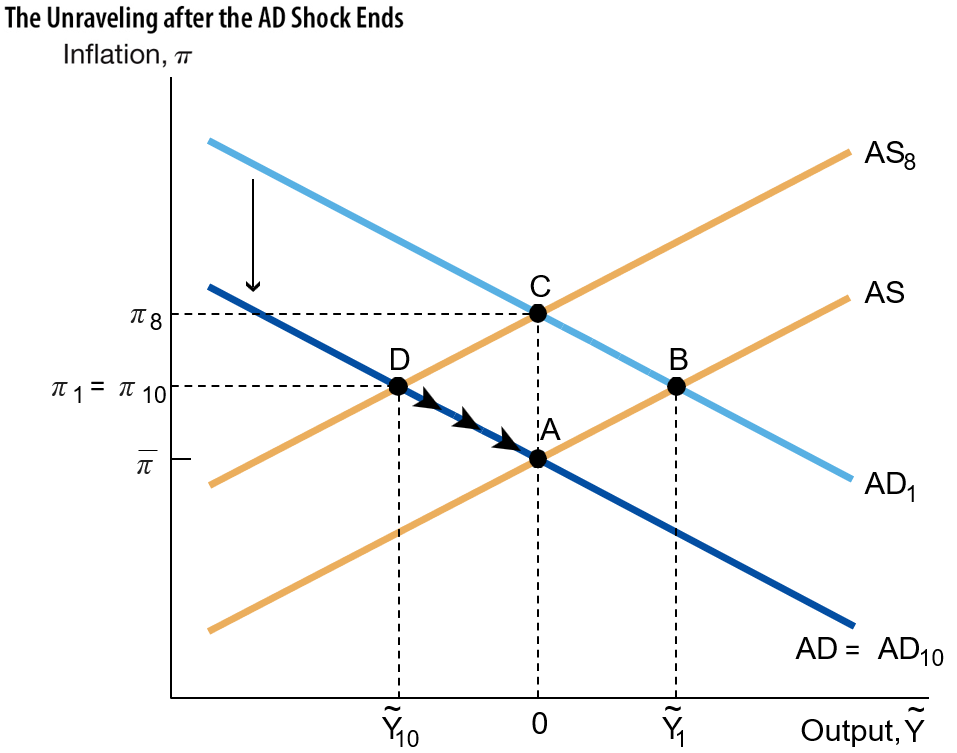
\includegraphics[width=0.5\linewidth]{Figures/fig_13_14}
	\end{center}
	
\end{frame}

\begin{frame}[wide]{Event 3: A Positive AD Shock}
	\begin{itemize}
		\item The AD shock implies that booms are matched by recessions
		\vspace{3mm}
		\begin{itemize}
			\item The economy benefits from a boom but inflation rises
			\item The way to reduce inflation is by a recession
		\end{itemize}
		\vspace{6mm}
		\item The costs of inflation: The economy would have been better off at the original steady state
	\end{itemize}
\end{frame}


\begin{frame}[wide]{Empirical Evidence: Predicting the Central Bank Policy Rate}
	\begin{itemize}
		\item Does simple monetary policy rule provides an accurate picture of the federal funds rate?
		\item Recall the policy rule and the Fisher's equation
		\[R_t - \bar{r} = \bar{m} \left(\pi_t -\bar{\pi}\right)\]
		\[i_t = R_t + \pi_t\]
		\item Use the Fisher equation to write the monetary policy rule in terms of the nominal interest rate:
		\[i_t = \bar{r} + \pi_t + \bar{m} \left(\pi_t -\bar{\pi}\right)\]
		\item It is commonly known as the Taylor's rule
		\vspace{2mm}
		\begin{itemize}
			\item The Taylor's rule typically also have output build into it
		\end{itemize}
	\end{itemize}
\end{frame}

\begin{frame}[wide]{The Fed Funds Rate, Actual and Predicted}
	\begin{itemize}
		\item Predicted level for the fed funds rate using the simple policy rule
		\begin{itemize}
			\item $\bar{m} =1/2, \bar{r} = 2\%, \bar{\pi}=2\%$ 
		\end{itemize}
		\item Some economists infer that monetary policy was excessively loose during 70s, resulting the high inflation in the 70s	
		\item The Fed also departs from the rule during recessions in the early 1990s, in the early 2000s, and since 2008
	\end{itemize}
	\begin{figure}
		\centering
		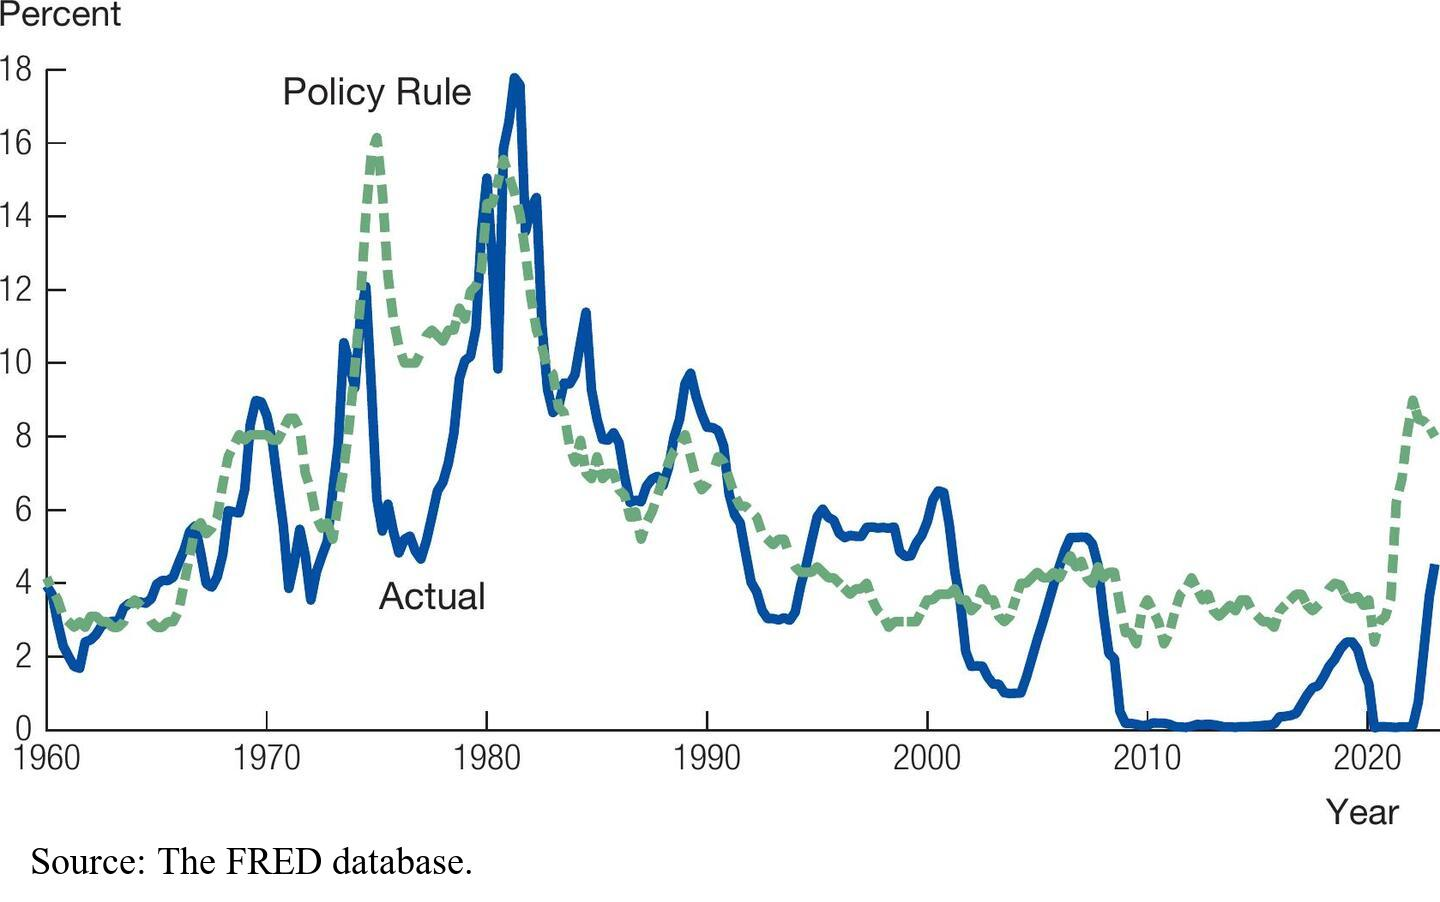
\includegraphics[width=0.55\linewidth]{Figures/MACRO6_FIG13.16}
	\end{figure}
	
\end{frame}

%\begin{frame}[wide]{Inflation-Output Loops}
%	\begin{itemize}
%		\item A prediction of the short-run model is that the economy follows counterclockwise loops 
%		\vspace{2mm}
%		\begin{itemize}
%			\item On a plot with the inflation rate on the vertical axis and output on the horizontal axis
%		\end{itemize}
%		\vspace{6mm}
%		\item Following a negative AD shock or to some degree a negative inflation shock, the economy would move in counterclockwise
%		\vspace{2mm}
%		\begin{itemize}
%			\item positive short-run output leads to rising inflation
%			\item a rise in inflation leads policymakers to reduce output
%		\end{itemize}
%	\end{itemize}
%\end{frame}
%
%\begin{frame}[wide]{Inflation-Output Loops in the U.S. Economy}
%	\begin{itemize}
%		\item This counterclockwise loop also appear in the data
%		\item The following traces the path of the years
%		\item A booming economy tends to raise inflation, high inflation is often followed by a recession to bring inflation down
%	\end{itemize}
%	\vspace{2mm}
%	\begin{figure}
%		\centering
%		\includegraphics[width=0.85\linewidth]{"Figures/fig 13_16"}
%	\end{figure}
%\end{frame}

%\begin{frame}[wide]{Forecasting and the Business Cycle}
%	\begin{itemize}
%		\item Economic forecasts are made regularly by ``professional" economists
%		\item Economists study a large number of economic variables that have proved useful in predicting the future path of the economy, called leading economic indicators
%		\begin{itemize}
%			\item Fed fund rates (FFR)
%			\item Term structure of interest rates
%			\item Unemployment claims
%			\item Number of new houses being built
%		\end{itemize}
%		\item More recently, people would use detail real-time data to make such forecast 
%		\begin{itemize}
%			\item At the moment, most aggregate data are reported quarterly. Economist cannot get data for Jan, and Feb until Q1 wrap up
%			\item e.g., Amazon may use its sale data to make prediction -- how much and what kind of item are consumer buying, etc
%		\end{itemize}
%		
%	\end{itemize}
%\end{frame}
%
%\begin{frame}[wide]{Forecasting and the Business Cycle}
%	\begin{itemize}
%		\item The bold line depicts the real trajectory of U.S. employment
%		\item Various trajectories are displayed based on the quarter of the forecast
%		\item During the Great Recession, forecasts consistently underestimated its severity
%	\end{itemize}
%	\begin{figure}
%		\centering
%		\includegraphics[width=0.5\linewidth]{"Figures/fig 13_17"}
%	\end{figure}
%	
%\end{frame}

%\begin{frame}[wide]{Modern Monetary Policy}
%	\begin{itemize}
%		\item The short-run model captures many features of monetary policy
%		\vspace{4mm}
%		\item Central banks are now more explicit about policies and targets but does not officially follow a monetary policy rule
%		\vspace{4mm}
%		\item Inflation rates in industrialized countries have been well-behaved for the last 25 years
%	\end{itemize}
%\end{frame}
%
%\begin{frame}[wide]{Inflation in the OECD}
%	\begin{itemize}
%		\item Overall, all countries in the OECD have been successful in maintaining low and stable inflation after the 80s
%		\item Some economists attribute the low inflation to good luck -- didn't experience oil shock like in the 70s. In fact, we faced a pandemic shock in 2020 but the central bank seem have deal with it well enough
%	\end{itemize}
%	\begin{figure}
%		\centering
%		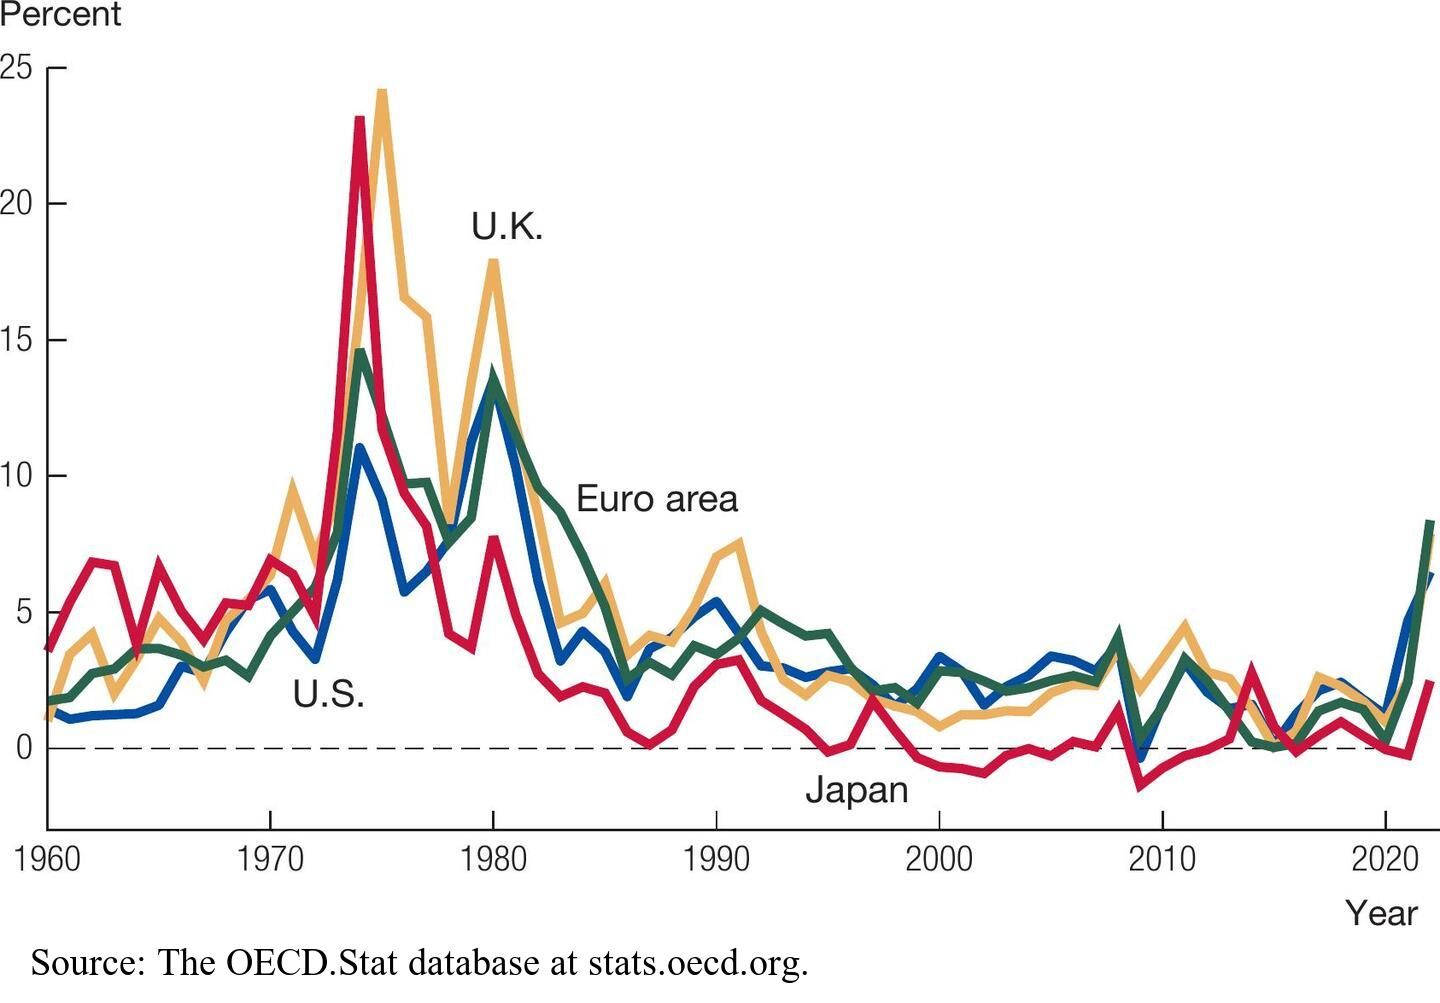
\includegraphics[width=0.55\linewidth]{Figures/MACRO6_FIG13.19}
%	\end{figure}
%	
%\end{frame}

%\begin{frame}[wide]{More Sophisticated Monetary Policy Rules}
%	
%	\begin{itemize}
%		\item Simple monetary policy rules suggest that interest rate changes depend only on inflation fluctuations
%		\item More sophisticated monetary policy rules incorporating short-run output, but it yields outcomes similar to the simpler model, as:
%		\begin{itemize}
%			\item The simple monetary policy implicitly accounts for output through the Phillips Curve
%			\item A positive correlation exists between inflation and short-run output
%			\item However, the simple rule only employs one parameter, $\bar{m}$, to determine the weight
%		\end{itemize}
%		\item While no central bank adheres strictly to a single rule, even more complicated ones, these rules may still offer guidance for monetary policymakers
%	\end{itemize}
%\end{frame}
%
%\begin{frame}[wide]{Rules versus Discretion}
%	\begin{itemize}
%		\item Too much information from the economy to cover with a single rule 
%		\item But, is there benefit following a systematic policy? Central bank may face time consistency problem
%		%		\begin{itemize}
%			%			\item 	Even though agents support a particular policy, once the future comes, they have incentives to renege on their promises
%			%		\end{itemize}
%		\item Due to high inflation, Central bank run a contractionary policy:
%		\begin{itemize}
%			\item Once firms and workers form inflation expectations, central bankers may pursue expansionary monetary policies to boost economic growth
%			\item However, firms and workers set prices anticipating these policies
%			\item Anticipating future policy moves, everyone strives to stay ahead, yielding no output benefits
%			\item Policymakers can maintain lower average inflation by committing to not exploiting firms' and workers' inflation expectations
%			\item An explicit and credible monetary policy rule achieves this effectively
%		\end{itemize}
%	\end{itemize}
%\end{frame}
%
%\begin{frame}[wide]{The Paradox of Policy and Rational Expectations}
%	\begin{itemize}
%		\item The goal of macroeconomic policy: full employment, output at potential, and most importantly low, stable inflation
%		
%		\item How might such a policy show up in our short-run model?
%		\begin{itemize}
%			\item A tough stance on inflation shows up in the monetary policy rule as a high value of m bar
%			\item The policymaker raises interest rates sharply in response to a modest increase in inflation, producing a large recession
%		\end{itemize}
%		\item The presence of a policymaker willing to generate a large recession to fight inflation makes policy use less likely  -- if that is something firm and household believe in 
%	\end{itemize}
%\end{frame}
%
%\begin{frame}[wide]{The Paradox of Policy and Rational Expectations}
%	\begin{itemize}
%		\item Under adaptive expectations, we assume 
%		\[\pi_t^e = \pi_{t-1}\]
%		\item Assume the equation does not change with policy rule changes
%		\begin{itemize}
%			\item This assumption may seem strange and too strong, as other factor are omitted, such as target rate of inflation
%			\item But, it is an easy way to introduce sticky inflation
%		\end{itemize}
%	\end{itemize}
%\end{frame}
%
%\begin{frame}[wide]{The Paradox of Policy and Rational Expectations}
%	\begin{itemize}
%		\item Rational expectations
%		\begin{itemize}
%			\item People use all information at their disposal to make their best forecast of the rate of inflation
%			\item But it may also include the central bank’s target rate of inflation ($\bar{\pi}$) and any announcements the bank may make about its future target 
%			\item So if a credible central bank changes its policy rule, expected inflation may adjust directly
%			\begin{itemize}
%				\item e.g., most previous Argentinian gov't claim they would bring down the hyperinflation, but the public does not believe they could or would do it... Any announcement had no effect on the inflation
%			\end{itemize}
%		\end{itemize}
%	\end{itemize}
%\end{frame}
%
%\begin{frame}[wide]{The Paradox of Policy and Rational Expectations}
%	\begin{itemize}
%		\item The central bank’s willingness to fight inflation is a key determinant of expected inflation
%		\item To the extent that policymakers can influence expectations, they can reduce the costs of maintaining a low target level of inflation
%		\vspace{2mm}
%		\begin{itemize}
%			\vspace{2mm}
%			\item If firms know the bank will fight aggressively to keep inflation low
%			\begin{itemize}
%				\vspace{2mm}
%				\item less likely to raise prices after an inflation shock
%			\end{itemize}
%			
%		\end{itemize} 
%	\end{itemize}
%\end{frame}
%
%\begin{frame}[wide]{Managing Expectations in the AS/AD Model}
%	\begin{itemize}
%		\item We can drop the assumption of adaptive expectations and rewrite the AS curve in terms of the expected rate of inflation:
%		\[\pi_{t+1} = \pi_t^e + \bar{\nu} \widetilde{Y}_t + \bar{o}\]
%		\item If the Federal Reserve lowers the inflation target, the AD curve shifts down through the interest rate
%		\item If expectations adjust immediately and people use all information, the AS curve shifts down immediately to the new target
%		\item If the central bank can control expectations of inflation, it can be kept low without recessions
%	\end{itemize}
%\end{frame}
%
%\begin{frame}[wide]{Costless Disinflation by Coordinating Expectations}
%	\begin{itemize}
%		\item The central bank lowers its target rate of inflation from 4 percent to 2 percent, shifting the AD curve back
%		\item Compare to the adaptive expectations, coordinating expected inflation can achieve low and stable inflation without recessions
%	\end{itemize}
%	\begin{figure}
%		\centering
%		\includegraphics[width=0.45\linewidth]{"Figures/fig 13_19"}
%	\end{figure}
%\end{frame}
%
%\begin{frame}[wide]{Rational Expectations and the Lucas Critique}
%	\begin{itemize}
%		\item The Lucas critique: argues that economic policy rules should be based on deep structural relationships in the economy, rather than statistical correlations observed in historical data
%		\begin{itemize}
%			\item Criticizes the use of empirical models based solely on historical data for policy analysis, as they may not accurately predict the effects of policy changes
%		\end{itemize}
%		\item The Lucas critique has had a profound impact on macroeconomic theory
%		\begin{itemize}
%			\item Modern models have internalized it
%			\item It incorporates the theory of rational expectations explicitly
%			\item The expectation modeling is still an active area of research
%			\begin{itemize}
%				\item e.g., robustness, rational inattention, etc
%			\end{itemize}
%		\end{itemize}
%	\end{itemize}
%\end{frame}

%\begin{frame}[wide]{Inflation Targeting}
%	How can central banks improve their management of inflation expectations?
%	\begin{itemize}
%		\item Announce an explicit monetary policy rule
%		\item Move in the direction of transparency, and adopt an explicit inflation target
%		\begin{itemize}
%			\item In the United States, the euro area, Japan, the United Kingdom, Australia, Brazil, Canada, Mexico, New Zealand, and Sweden, central banks are not required to deliver the target rate of inflation in every period, but they all have regular meeting over a reasonable time frame (6 weeks or so)
%		\end{itemize}
%		\item This helps anchor inflation expectations
%		\item Many countries have an explicit inflation target that they seek to apply over the medium horizon
%		\item Yet, they should have constrained discretion: maintaining flexibility to respond to shocks with a commitment to particular inflation rate in the long run
%		
%	\end{itemize}
%\end{frame}

%\begin{frame}[wide]{An Increase in the Investment Rate}
%	\begin{columns} 
%			% Column 1
%			\begin{column}{.5\textwidth}
%				\begin{itemize}
%					\item Suppose the investment rate increases permanently for exogenous reasons ($s'>s$)
%					\begin{itemize}
%						\item The investment curve rotates upward ($\bar{s}'\bar{A}  \bar{L}^{1-\alpha} K_t^\alpha > \bar{s}\bar{A}  \bar{L}^{1-\alpha} K_t^\alpha$)
%						\item The depreciation curve remains unchanged ($\delta K_t$)
%						\item The capital stock increases by transition dynamics to reach the new steady state
%						\begin{itemize}
%							\item This happens because investment exceeds depreciation ($sY_t>\delta K_t$)
%						\end{itemize}
%						\item The new steady state is located to the right
%					\end{itemize}
%				\end{itemize}
%			\end{column}
%			% Column 2    
%			\begin{column}{.5\textwidth}			
%				\begin{figure}
%					\centering
%					\includegraphics[width=1\linewidth]{"Figures/An Increase in the Investment Rate"}
%				\end{figure}
%			\end{column}%
%		\end{columns}
%\end{frame}

%\begin{frame}[wide]{Measuring the State of the Economy}
%	\begin{columns} 
%		% Column 1
%		\begin{column}{.5\textwidth}
%			\begin{table}[htbp]
%				\centering
%				\begin{tabular}{lrrrr}
%					& 2005  & 2006  & 2007  & 2008 \\
%					\hline
%					GDP   & 12.6  & 13.4  & 14.0    & 14.3 \\
%					(in trillions of \$) &       &       &       &  \\
%					Growth rate GDP &       & 0.063 & 0.045 & 0.021 \\
%					\hline
%				\end{tabular}%
%				\label{tab:addlabel}%
%			\end{table}%
%		\end{column}
%		% Column 2    
%		\begin{column}{.5\textwidth}			
%			
%			
%		\end{column}%
%	\end{columns}
%\end{frame}

\begin{frame}[wide]{Next Lecture}
	\begin{itemize}
		\item Next Lecture will cover Ch.18
	\end{itemize}
\end{frame}

\end{document}